\documentclass[12pt]{article}

% packages
\usepackage{graphicx}
\usepackage{hyperref}
\usepackage{amsmath}
\usepackage{amssymb}
\usepackage{natbib}
\usepackage{apalike}

% title
\title{Cuestionario 2: The Nature of the Colonized}

% include authors file
\input{authors.authors}

\date{April 28, 2023}




\begin{document}

% title page
\maketitle

\newpage

% table of contents
\tableofcontents

\newpage

% abstract (optional)
\begin{abstract}
Provide the literature on the political, economic, and cultural features prescribed in the fragebogen. 
\end{abstract}





\section{Ancient Philippine Society}
  \subsection{Location of the Philippines}
  The Philippines is a country located in Southeast Asia. It is a part of the nations in Southeast Asia forming a fully opened fan \citep{corpuz1965philippines}. 
  It is in the south of Taiwan, north of Indonesia, and east of Vietnam. The islands are located between bodies of water such as the South China Sea 
  on the left and the Pacific Ocean on the right. In the map, the country is situated at \textbf{14.5995° N} latitude and \textbf{120.9842° E} longitude.
  \begin{figure}[htbp]
    \centering
    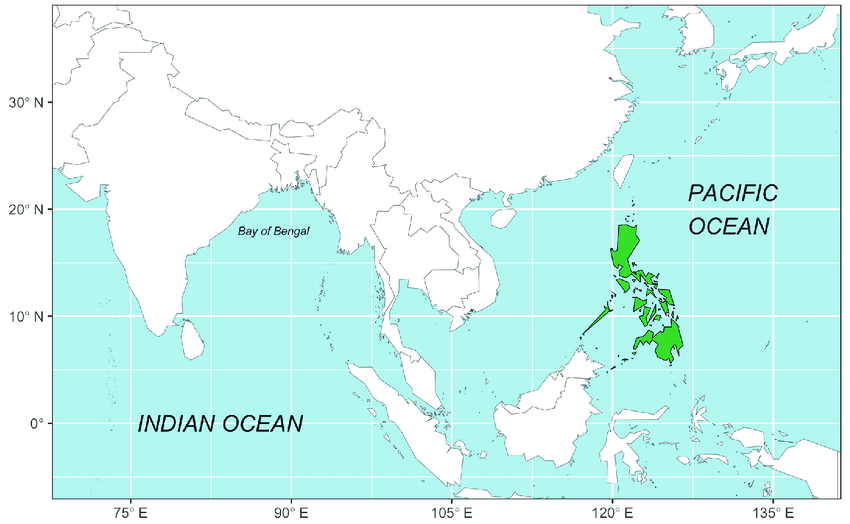
\includegraphics[width=1\textwidth]{images/1_1-philippine_map.png}
    \caption{Map Location of Philippines. (Source: R maptool package)}
    \label{fig:image}
  \end{figure}

  \subsection{Prominent Features of the Philippines}
  Philippines have more than 7,000 islands and islets that stretched around 1,600 kilometers from north to south. It also have a lot of mountains, an extensive but small
  river system, occassional small earthquakes that roughly happened around 22 times a day because Philippines lies above the Pacific Ring of Fire, it is also heavily affected
  by typhoons because it is close to the coastal line in which the east side of it is the Pacific Ocean, and Philippines is bountiful of natural resources that
  has never yet been extracted. (\citeauthor{agoncillo1990filipino}, \citeyear{agoncillo1990filipino}, pp. 1-3; \citeauthor{foreman1899islands}, \citeyear{foreman1899islands}, pp. 5-6, 14-16)
   
  \subsection{Philippines' Encounter with Spain}
  Philippines encountered Spain because of the voyages brought by the Spaniards in order to develop a world economic system. This was when Legazpi aimed to sail
  to the Philippines. This is also where Magellan encountered Lapu-Lapu at that time. During this time, Spain thought of implementing the same mercantilist system
  commanded by the capitalistic big empire of Europe. By exploring to other countries, its purpose was to acquire resources and labor to further develop
  capitalism so that they can profit more. (\citeauthor{constantino1975history}, \citeyear{constantino1975history}, pp. 15-16)
  

  \subsection{The Balangay}
  sdf






\section{Political Institutions Introduced by Spain}
Insert background information here.






\section{Economic Institutions Introduced by Spain}
Insert methodology here.





\section{Cultural Institutions Introduced by Spain}
Insert results here.






% references
\bibliographystyle{apalike}
\bibliography{references}

\end{document}
